\label{sec:object_detection}

Object detection is one of the subtasks in the image domain.
It is an extension of the classification task, where additionally to the predicted class, the location of the objects in the image should be predicted.
The location is normally given as a bounding box, where throughout this thesis the bounding box format by Redmon et al. \cite{yolov1} is used to label object instances.
In this format a bounding box is defined as:

\begin{equation}
    bbox = (x_{rel}, y_{rel}, w_{rel}, h_{rel})
\end{equation}

Where the bounding box is presented as a tuple of four values.
The first two values indicate the center of the bounding box relative to the image size, while the latter two values indicate the width and the height of the bounding box also relative to the image size.
All values can be calculated by dividing the absolute value by the corresponding image value.
For example $x_{rel}$ would be calculated by dividing the absolute x-coordinate $x_{abs}$ by the width of the image.
Same applies for $y_{rel}$, except here the value is divided by the image height.
$w_{rel}$ and $h_{rel}$ are calculated following the same principles.
The advantages of this format are, that the definition of the bounding box becomes invariant to the image size.
The image can be resized without having to recalculate the bounding box, as it is the case with other formats which use an absolute definition for bounding boxes.

\subsection{History of Object Detection}
\label{sec:hostory_obj_detection}

\subsubsection{Sliding Window}
The simplest algorithm to detect objects in an image is the sliding window approach.
A classifier is trained on image patches which contain the object to detect.
To now detect the objects in an unseen image, the image is divided into patches of various scale and fed to the classifier.
The prediction score of the patches is thresholded with a predefined value.
High confidence patches are likely to contain an object and are kept \cite{sliding_window_satelite}.

% Before an object detection can be performed on an image, a classifier has to be trained.
% This classifier is normally trained on image patches, where a patch has roughly the size of the objects it should classify.
% The object detection phase starts by dividing the input image into patches.
% Those patches are now fed to the classifier and when the predicted probability exceeds a predefined threshold the patch is considered to have an object in it.
% It should be noted that classification accuracy can be improved by feeding overlapping patches into the classifier.
% The resulting predicted bounding boxes now look like the image on the left side in fig. \ref{fig:nms_before_after}.
% It contains multiple bounding boxes for the same object.
% To have only one prediction per object, a \ac{NMS} algorithm is applied on the overlapping bounding boxes.
% The most common \ac{NMS} algorithm is the greedy-\ac{NMS}.
% Here bounding boxes are grouped together, when their overlap exceeds a certain threshold.
% Rejection of neighboring bounding boxes is done by using the predicted class probability i.e. using only those bounding boxes with the highest prediction score and rejecting the others \cite{learn_nms}.
% The results of a \ac{NMS} can be seen on the right side in fig. \ref{fig:nms_before_after}.


% - TODO add tackle scale by using patches of different size

% \begin{figure}
% \begin{center}
%     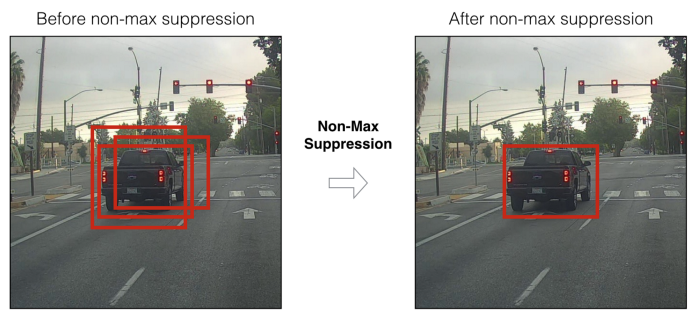
\includegraphics[width=10cm]{imgs/nms_before_after.png}
%     \caption{Predicted bounding boxes before and after a non-maximum suppression was applied \cite{nms_before_after}}
%     \label{fig:nms_before_after}
% \end{center}
% \end{figure}

\subsubsection{Regions with CNN Features (R-CNN)}
While the sliding window approach is effective, it is also highly inefficient, since every generated patch has to be processed by the classifier in order to find all possible objects in an image.
\ac{R-CNN} by Girshick et al. \cite{rcnn} improves on that by using a region proposal algorithm to obtain probable regions of an object.
In their work the Selective Search algorithm \cite{selective_search} was used to generate region proposals.
How the algorithm performs and what kind of bounding boxes are produced, can be seen in fig. \ref{fig:selective_search}.
$2000$ of those proposed bounding boxes are taken from different scales and warped into the input shape of the following \ac{CNN}, disregarding the size or aspect ratio of the proposed bounding box.
Each of the bounding boxes is separately passed through the \ac{CNN} and yields a feature vector which is classified by $N + 1$ binary \acp{SVM} ($N$ classes $+1$ general background class) to produce the class prediction.
Further, the bounding box is improved through $N$ separately trained bounding box regressor \acp{SVM} \cite{bbox_regressor}.

\begin{figure}
\begin{center}
    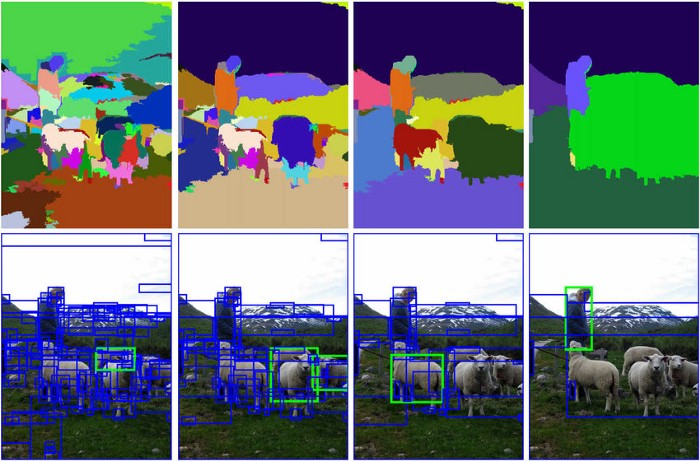
\includegraphics[width=10cm]{imgs/selective_search.png}
    \caption{Example of results obtained through the Selective Search algorithm (top) with increasing region scale from left to right and bounding boxes drawn around those regions (bottom). Selective Search produces sub-segmentations of objects in an image, considering size, color, texture and shape based features for the grouping of the regions \cite{selective_search}.}
    \label{fig:selective_search}
\end{center}
\end{figure}

\subsubsection{Fast R-CNN}
While \ac{R-CNN} was an improvement to the previous methods, the training and inference process was still very expensive, since it involved multiple stages.
With Fast R-CNN Girshick \cite{fast_rcnn} improved on the training and inference time by a large margin in contrast to \ac{R-CNN}.

The main difference to \ac{R-CNN} is that instead of generating region proposals and passing them through the \ac{CNN}, region proposals are now projected onto the feature maps of the \ac{CNN} and pooled into a fixed size grid through a \ac{RoI} pooling layer.
Meaning that the \ac{CNN} computations are shared between each bounding box proposal resulting in a drastic inference speed improvement.
After pooling, the \ac{RoI} it is processed by a fully-connected layer, producing a so called \ac{RoI} feature vector.
This feature vector is fed into a siblings output layer.
The first branch is a classification layer with a softmax output, producing class probabilities and replaces the previous \acp{SVM}.
The second branch is comprised of a bounding box regression layer, which outputs bounding box regression offsets as in \ac{R-CNN} \cite{rcnn}.
% Due to the one-stage nature of the pipeline a novel multi-task loss was required,
% which the author defined as follows:

% \begin{equation}
%     L(\hat{y}, y, \hat{b}, b) = L_{cls}(\hat{y}, y) + \lambda L_{loc}(\hat{b}, b)
% \end{equation}

% $\hat{y}$ being the predicted class probabilities by the softmax layer and $y$ the ground truth class.

% - TODO should I even do that further?

% \subsubsection{Faster R-CNN}

% In Fast \ac{R-CNN} the prediction time was decreased by compressing the multi-stage pipeline into a single-stage pipeline.
% The remaining non-learnable part of the pipeline became the region proposal algorithm.
% It still took around $2s$ to propose bounding boxes with Selective Search.
% Ren et. al therefore proposed Faster \ac{R-CNN} \cite{faster_rcnn} to further increase the performance of the overall algorithm.
% In Faster \ac{R-CNN} the performance is boosted through the novel \ac{RPN}.
% As with Fast \ac{R-CNN} an image is first fed to the \ac{CNN} to produce feature maps.
% Afterwards, the feature maps are used as an input to the \ac{RPN}, which operates in a sliding window fashion, where a window size of $nxn$ ($n = 3$) is used to traverse the whole feature map and produce features for the following network.

\subsubsection{Anchor Box Based Single Shot Detectors}

Various object detection networks such as, Faster \ac{R-CNN} \cite{faster_rcnn}, \ac{YOLO} \cite{yolov1}, \ac{SSD} \cite{ssd} and RetinaNet \cite{focalloss} use anchor boxes to predict the objects in an image.
Further, all the named methods predict the class as well as the bounding boxes for the objects in a single network pass, therefore the name single shot.
Anchor boxes are predefined boxes of various size aspect ratio, which are used as a base for the prediction bounding box prediction of the above networks.
Instead of making the network predict the bounding box directly, the network predicts bounding box regression offsets based on a certain anchor box \cite{yolov3}.
The selection of good anchor box sizes is a hyperparameter in the training of an object detector and can improve the prediction quality \cite{faster_rcnn}.
The scale and aspect ratio of the anchor boxes is often selected by using the k-means clustering algorithm on the labeled bounding boxes of the dataset \cite{yolov2}.


% Anchor boxes are used to assign a ground truth to a prediction of a network, which is then used to apply a loss on the prediction and hence make the network learn.
% For example in Faster \ac{R-CNN} the ground truth bounding box is assigned to an anchor when the \ac{IoU} of the bounding box and the anchor box is greater than a certain threshold.
% Anchor boxes can be seen as predictors, who over time get better and better of predicting objects of certain size and aspect ratios \cite{yolov1}.


\subsubsection{Anchor Box Free Single Shot Detectors}

Another class of single shot detectors are the anchor box free detectors such as \ac{YOLOv1} \cite{yolov1}, CornerNet \cite{corner_net}, CenterNet \cite{center_net} and the \ac{FCOS} \cite{fcos}.
The advantages of anchor box free detection methods are that complicated computation related to anchor boxes, e.g. calculating the \ac{IoU} at training time, can be omitted \cite{fcos}, as well as the tuning of anchor box sizes for the specific task \cite{center_net}.
As of now, all the above methods perform worse than their current state-of-the-art anchor box based counterparts \cite{yolov4}.



\subsection{Intersection Over Union (IoU)}

The \ac{IoU}, which is also known as the Jaccard index, is a measure for how much two arbitrary shapes (volumes) are overlapping \cite{giou}.
In object detection \ac{IoU} is often used to compare two bounding boxes $A$ and $B$ and also to construct various loss functions as well as metrics.

\begin{equation}
    \text{IoU}(A, B) = \frac{|A \cap B|}{|A \cup B|} = \frac{| A \cap B |}{|A| + |B| - |A \cap B|}
\end{equation}


\subsection{IoU Based Loss Functions}

The \ac{MSE} has shown to perform not well for the task of bounding box regression, because it assumes that the regressed variables ($x$, $y$, $w$, $h$) are independent of each other and can be optimized separately \cite{iou}.

To take the correlation of those variables into account, Yu et al. \cite{iou} proposed the \ac{IoU} loss (equation \ref{eq:iou_loss}).
While this was a major improvement to previously known methods the \ac{IoU} loss still suffers from slow convergence and from the gradient vanishing problem, which occurs when the two bounding boxes $A$ and $B$ have no intersection.

\begin{equation}
    \text{L}_{\text{IoU}}(A, B) = 1 - \text{IoU}(A, B)
    \label{eq:iou_loss}
\end{equation}

Further, to solve these drawbacks Rezatofighi et al. \cite{giou} proposed the \ac{GIoU} loss (equation \ref{eq:giou_loss}).
Their loss introduces an additional penalty term added to the \ac{IoU} loss.
Here, $C$ is the smallest convex box enclosing $A$ and $B$.
Hence, when the boxes have no overlap there is still a gradient pushing them closer to each other.
While the \ac{GIoU} loss is a major improvement in terms of vanishing gradient, it suffers from slow convergence when $A$ and $B$ have overlap and at the same time $A$ contains $B$ (or vice versa), because the penalty term then becomes $0$, as a consequence the \ac{GIoU} loss becomes the \ac{IoU} loss.
Furthermore, it has been observed that when $A$ and $B$ have no overlap, instead of decreasing the spatial distance between $A$ and $B$, the \ac{GIoU} loss tends to increase the size of the bounding box area to reduce the loss \cite{eiou}.

\begin{equation}
    \text{L}_{\text{GIoU}}(A, B) = 1 - \text{IoU}(A, B) + \frac{|C - (A \cup B)|}{|C|}
    \label{eq:giou_loss}
\end{equation}

The next improvement in the \ac{IoU} based loss function space was proposed by Zheng et al. \cite{diou}, with their \ac{DIoU} and \ac{CIoU} loss functions.
In contrast to \ac{GIoU}, \ac{DIoU} (equation \ref{eq:diou_loss}) solves the gradient vanishing problem by considering the normalized distance of the central points of the two bounding boxes.
The squared euclidean distance is normalized by the squared diagonal length of the smallest box containing $A$ and $B$.

\begin{equation}
    \text{L}_{\text{DIoU}}(A, B) = 1 - \text{IoU}(A, B) + \frac{\|(A_{center} - B_{center})\|^2}{\|C_{diag}\|^2}
    \label{eq:diou_loss}
\end{equation}

To further improve on that, the authors additionally considered the aspect ratio of the bounding box to be another important geometric factor for bounding box regression.
Hence, the \ac{DIoU} loss is further extended by a penalty term considering the aspect ratio and resulting in the improved \ac{CIoU} loss (equations \ref{eq:ciou_loss}, \ref{eq:ciou_nu}, \ref{eq:ciou_alpha}).

The penalty in \ac{CIoU} is split into $\alpha$ and $\nu$.
The term $\alpha$ is a trade-off parameter which gives higher priority to the overlapping factor, especially in the case of non-overlap.
Further, $\nu$ is the parameter penalizing the difference in the aspect ratios of $A$ and $B$.
Still, it can be noticed that $\nu$ is $0$ when the aspect ratios are the same, regardless of the underlying relations between $A_w$, $B_w$ and $A_h$, $B_h$.
E.g. the aspect ratio is the same for all boxes with the following property $\{ (A_w=kB_w, \ A_h=kB_h)\ |\ k \in \R^+\}$ \cite{eiou}.

\begin{equation}
    \text{L}_{\text{CIoU}}(A, B) = \text{DIoU}(A, B) + \alpha(A,B) \cdot \nu(A, B)
    \label{eq:ciou_loss}
\end{equation}

\begin{equation}
    \nu(A, B) = \frac{4}{\pi^2} \left[arctan\left(\frac{A_w}{A_h}\right) - arctan\left(\frac{B_w}{B_h}\right)\right]^2
    \label{eq:ciou_nu}
\end{equation}

\begin{equation}
    \alpha(A, B) = \frac{\nu}{1 - IoU(A, B) + \nu'}
    \label{eq:ciou_alpha}
\end{equation}

Therefore, Zhang et al. \cite{eiou} proposed the \ac{EIoU} loss to remove this error.
The aspect ratio penalty is here replaced through two separate penalties, which consider the normalized width and height of the two bounding boxes.

\begin{equation}
    \text{L}_{\text{EIoU}}(A, B) = 1 - IoU(A, B) + \frac{\|(A_{center} - B_{center})\|^2}{\|C_{diag}\|^2} + \frac{\|(A_{w} - B_{w})\|^2}{\|C_w\|^2} + \frac{\|(A_{h} - B_{h})\|^2}{\|C_h\|^2}
    \label{eq:eiou_loss}
\end{equation}
